%This is a Tex Version of NE 806 Homework Template
%
\documentclass{amsart}
\setlength{\textheight}{9in}
\setlength{\topmargin}{-0.25in}
\setlength{\textwidth}{7in}
\setlength{\evensidemargin}{-0.25in}
\setlength{\oddsidemargin}{-0.25in}
\usepackage{amsfonts}
\usepackage[utf8]{inputenc}
\usepackage[T1]{fontenc}
\usepackage{graphicx} 
\usepackage[export]{adjustbox}
% needed to include these graphics
%\graphicspath{{./Pictures/}}      % only in case you want to keep the pictures in a separate
                                  % subdirectory; also see the appropriate line below
\usepackage{caption}
\usepackage{subcaption}
\usepackage{float}
\usepackage{framed}
\newcounter{temp}
\theoremstyle{definition}
\newtheorem{Thm}{Theorem}
\newtheorem{Prob}{Problem}
\newtheorem*{Def}{Definition}
\newtheorem*{Ans}{Answer}
\newcommand{\dis}{\displaystyle}
\newcommand{\dlim}{\dis\lim}
\newcommand{\dsum}{\dis\sum}
\newcommand{\dint}{\dis\int}
\newcommand{\ddint}{\dint\!\!\dint}
\newcommand{\dddint}{\dint\!\!\dint\!\!\dint}
\newcommand{\dt}{\text{d}t}
\newcommand{\dA}{\text{d}A}
\newcommand{\dV}{\text{d}V}
\newcommand{\dx}{\text{d}x}
\newcommand{\dy}{\text{d}y}
\newcommand{\dz}{\text{d}z}
\newcommand{\dw}{\text{d}w}
\newcommand{\du}{\text{d}u}
\newcommand{\dv}{\text{d}v}
\newcommand{\ds}{\text{d}s}
\newcommand{\dr}{\text{d}r}
\newcommand{\dth}{\text{d}\theta}
\newcommand{\bbR}{\mathbb{R}}
\newcommand{\bbN}{\mathbb{N}}
\newcommand{\bbQ}{\mathbb{Q}}
\newcommand{\bbZ}{\mathbb{Z}}
\newcommand{\bbC}{\mathbb{C}}
\newcommand{\dd}[2]{\dfrac{\text{d}#1}{\text{d}#2}}
\newcommand{\dydx}{\dfrac{\text{d}y}{\text{d}x}}
\renewcommand{\labelenumi}{{\normalfont \arabic{enumi}.}}
\renewcommand{\labelenumii}{{\normalfont \alph{enumii}.}}
\renewcommand{\labelenumiii}{{\normalfont \roman{enumiii}.}}
\font \bggbf cmbx18 scaled \magstep2
\font \bgbf cmbx10 scaled \magstep2
\usepackage{fancyhdr}
\usepackage{lipsum}
\usepackage{amsmath}
\usepackage{empheq}
\newcommand*\widefbox[1]{\fbox{\hspace{2em}#1\hspace{2em}}}
% Clear the header and footer
\fancyhead{}
\fancyfoot{}
% Set the right side of the footer to be the page number
\rfoot{\thepage}
\fancyhf{}
\pagestyle{fancy}
\begin{document}
\LARGE{NE-806: Neutronics}
 
\large
Homework \#4 due Thurs. November 15th, 2018
 
Solutions by: John Boyington
\newline
\bigskip


%%%%%%%%%%%%%%%%%%%%%%%%%%%%%%%%%%%%%%%%%%%%%%%%%%%%%%%%%%%%%%%%%%%%%%%%%%%%%%%%%%%%%%%%%%%%%%%%%%%%%%%%%%%%%%%%%%%%%%%%%%%
%                                                         PROBLEM 1
%%%%%%%%%%%%%%%%%%%%%%%%%%%%%%%%%%%%%%%%%%%%%%%%%%%%%%%%%%%%%%%%%%%%%%%%%%%%%%%%%%%%%%%%%%%%%%%%%%%%%%%%%%%%%%%%%%%%%%%%%%%

\textbf{Problem 1:} \newline For the following one-speed diffusion problems write: (1) the appropriate from of the diffusion equation (with a sketch showing the problem geometry), (2) the form of the most general solution (including any particular solution), (3) the boundary/source conditions you would use to find values for any arbitrary constants in your general solution, and (4) an explicit expression for the flux density.
Assume a vacuum surrounds the media.
\bigbreak

(a) An infinite homogeneous slab of thickness $T$ has a volumetrically distributed source with a strength $S(x)$ = $S_0x^2$ neutrons $cm^3$ $s^{-1}$ where $x$ is measured from the left surface of the slab.\newline
\bigbreak

(b) An infinite homogeneous cylinder of diameter $T$ contains a uniformly distributed source of strength $S_0$ neutrons $cm^{-3}$ $s^{-1}$.\newline
\bigbreak

(c) A homogeneous sphere of diameter $T$ contains a uniformly distributed source of strength $S_0$ neutrons $cm^{-3}$ $s^{-1}$.\newline
\bigbreak

(d) Two infinite homogeneous slabs each of thickness $T$ are placed a distance $T$ apart.
The left slab has a distributed source $S(x)$ = $S_0\cos \alpha x$ neutrons $cm^{-3}$ $s^{-1}$ where $x$ is measured from the outer surface.
The outer surface of the other slab is illuminated uniformly by a perpendicular neutron beam of strength $I_0$ neutrons $cm^{-2}$ $s^{-1}$.\newline
\bigbreak

%%%%%%%%%%%%%%%%%%%%%%%%%%%%%%%%%%%%%%%%%%%%%%%%%%%%%%%%%%%%%%%%%%%%%%%%%%%%%%%%%%%%%%%%%%%%%%%%%%%%%%%%%%%%%%%%%%%%%%%%%%%
\textbf{Solution}
\bigbreak
(a) The approximate form of the diffusion equation for a infinite slab reactor is given below:
\bigbreak


\begin{equation*}
    \frac{d^2}{dx^2}\phi(x) + B^2\phi(x) + \frac{S(x)}{D} = 0
\end{equation*}
 
\begin{figure}[h!]
    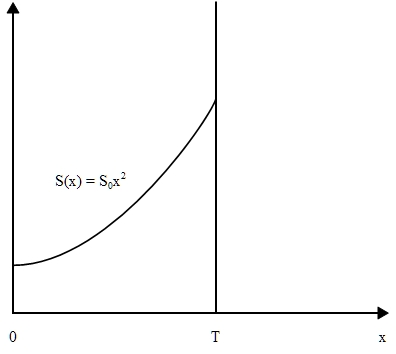
\includegraphics[width=.45\linewidth]{P1a}
\end{figure}
\bigbreak


Shown below is the form of the general solution:
\bigbreak

\[   \phi(x) = \left\{
\begin{array}{ll}
      Ae^{-Bx} + Ce^{Bx} &  \\
      A'\sinh(Bx) + C'\cosh(Bx) &  \\
\end{array}
\right. , \quad B^2 < 0\]
\bigbreak

\[   \phi(x) = \left\{
\begin{array}{ll}
      Ae^{-iBx} + Ce^{iBx} &  \\
      A'\sin(Bx) + C'\cos(Bx) &  \\
\end{array}
\right. , \quad B^2 > 0\]
\bigbreak


And here we see the boundary conditions for this geometry:
\begin{itemize}
    \item $J^+$(0) = 0
    \item $J^-$(T) = 0
\end{itemize}
\bigbreak


The homogeneous solution can be found using the general form:
\begin{equation*}
    \phi_h(x) = Ae^{-Bx} + Ce^{Bx}
\end{equation*}


And then the particular solution is obtained:
\begin{equation*}
    \phi_p(x) = \frac{2\frac{S_0}{D}}{(B^2)^2} + \frac{\frac{S_0}{D}x^2}{B^2}
\end{equation*}


Apply BC1:
\begin{equation*}
    J^\mp(x) = \frac{\phi(x)}{4} \pm \frac{D}{2} \phi'(x)
\end{equation*}


This allows us to obtain an equation that relates $A$ to $C$:
\begin{align*}
     0 &= J^+(0) = \frac{\phi(0)}{4} - \frac{D}{2} \phi'(0) \\
     0 &= 0.25\bigg[\frac{2\frac{S_0}{D}}{(B^2)^2}+A+C\bigg] - \frac{D}{2}\bigg[AB-CB\bigg] \\
     0 &= \bigg[\frac{2\frac{S_0}{D}}{(B^2)^2}+A+C\bigg] - 2D\bigg[AB-CB\bigg] \\
     0 &= A[1-2DB] + C[1+2DB]+\frac{2\frac{S_0}{D}}{(B^2)^2} \\
     A[2DB-1] &= C[1+2DB]+\frac{2\frac{S_0}{D}}{(B^2)^2} \\
     A &= \frac{-C(1+2DB)-\frac{2\frac{S_0}{D}}{(B^2)^2}}{1-2DB}
\end{align*}


Apply BC2:
\begin{align*}
     0 &= J^-(T) = \frac{\phi(T)}{4} + \frac{D}{2} \phi'(T) \\
     0 &= \bigg[\frac{2\frac{S_0}{D}}{(B^2)^2} + \frac{\frac{S_0}{D}T^2}{B^2}+\frac{4DT\frac{S_0}{D}}{B^2}\bigg] + A(e^{BT})[1+2DB]+C(e^{-BT})[1-2DB]
\end{align*}


Substitute $A$:
\begin{align*}
    0 &= \bigg[\frac{2\frac{S_0}{D}}{(B^2)^2} + \frac{\frac{S_0}{D}T^2}{B^2}+\frac{4DT\frac{S_0}{D}}{B^2}\bigg] + \frac{-C(1+2DB)-\frac{2\frac{S_0}{D}}{(B^2)^2}}{1-2DB}(e^{BT})[1+2DB]+C(e^{-BT})[1-2DB] \\
    0 &= C\bigg[(e^{-BT})[1-2DB] - \frac{1+2DB}{1-2DB}(e^{BT})[1+2DB]\bigg] +\bigg[\frac{2\frac{S_0}{D}}{(B^2)^2} + \frac{\frac{S_0}{D}T^2}{B^2}+\frac{4DT\frac{S_0}{D}}{B^2} - \frac{\frac{2\frac{S_0}{D}}{(B^2)^2}}{1-2DB}\bigg] \\
    C &= \frac{\bigg[\frac{\frac{2\frac{S_0}{D}}{(B^2)^2}(e^{BT})[1+2DB]}{1-2DB} - \frac{2\frac{S_0}{D}}{(B^2)^2} - \frac{\frac{S_0}{D}T^2}{B^2}-\frac{4DT\frac{S_0}{D}}{B^2} \bigg]}{\bigg[(e^{-BT})[1-2DB] - \frac{1+2DB}{1-2DB}(e^{BT})[1+2DB]\bigg]}
\end{align*}


\begin{equation*}
    A = \frac{-\frac{\bigg[\frac{\frac{2\frac{S_0}{D}}{(B^2)^2}(e^{BT})[1+2DB]}{1-2DB} - \frac{2\frac{S_0}{D}}{(B^2)^2} - \frac{\frac{S_0}{D}T^2}{B^2}-\frac{4DT\frac{S_0}{D}}{B^2} \bigg]}{\bigg[(e^{-BT})[1-2DB] - \frac{1+2DB}{1-2DB}(e^{BT})[1+2DB]\bigg]}(1+2DB)-\frac{2\frac{S_0}{D}}{(B^2)^2}}{1-2DB}
\end{equation*}


And the following equation is for the flux in the slab:
\begin{empheq}[box=\widefbox]{align*}
    \phi(x) &= \frac{-\frac{\bigg[\frac{\frac{2\frac{S_0}{D}}{(B^2)^2}(e^{BT})[1+2DB]}{1-2DB} - \frac{2\frac{S_0}{D}}{(B^2)^2} - \frac{\frac{S_0}{D}T^2}{B^2}-\frac{4DT\frac{S_0}{D}}{B^2} \bigg]}{\bigg[(e^{-BT})[1-2DB] - \frac{1+2DB}{1-2DB}(e^{BT})[1+2DB]\bigg]}(1+2DB)-\frac{2\frac{S_0}{D}}{(B^2)^2}}{1-2DB}e^{-Bx} \\ &+ \frac{\bigg[\frac{\frac{2\frac{S_0}{D}}{(B^2)^2}(e^{BT})[1+2DB]}{1-2DB} - \frac{2\frac{S_0}{D}}{(B^2)^2} - \frac{\frac{S_0}{D}T^2}{B^2}-\frac{4DT\frac{S_0}{D}}{B^2} \bigg]}{\bigg[(e^{-BT})[1-2DB] - \frac{1+2DB}{1-2DB}(e^{BT})[1+2DB]\bigg]}e^{Bx} +\frac{2\frac{S_0}{D}}{(B^2)^2} + \frac{\frac{S_0}{D}x^2}{B^2}
\end{empheq}


%###############################################################################
% section (b)
%###############################################################################

\bigbreak
b) The approximate form of the diffusion equation for a infinite cylinder reactor is given below:
\bigbreak

\begin{equation*}
    \frac{d^2}{dr^2}\phi(r) + \frac{1}{r}\frac{d}{dr}\phi(r) +B^2\phi(r) + \frac{S(r)}{D} = 0
\end{equation*}

\begin{figure}[h!]
    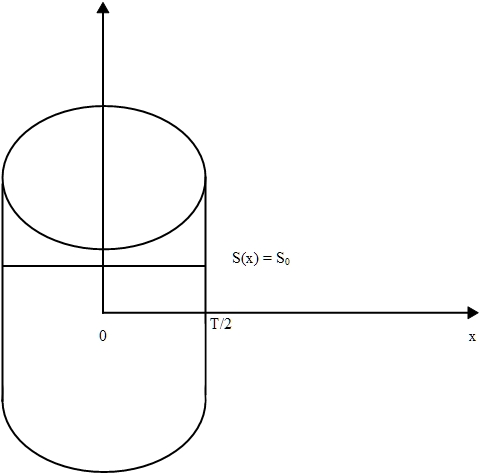
\includegraphics[width=.45\linewidth]{P1b}
\end{figure}
\bigbreak


Below is the general form of the solution:
\bigbreak
\[   \phi(r) = \left\{
\begin{array}{ll}
      AI_0(Br) + CK_0(Br), &  B^2 < 0\\
      AJ_0(Br) + CY_0(Br), &  B^2 > 0\\
\end{array}
\right. \]
\bigbreak


And these are the boundary conditions:
\begin{itemize}
    \item $\phi(0) \neq \infty$
    \item $J^-$(T/2) = $J^+$(-T/2) = 0
    \item $\lim_{x\to\infty} \phi(x)$ = 0
\end{itemize}


Apply BC1:
\begin{equation*}
    \phi(0) \neq \infty, \quad so \quad C = 0
\end{equation*}

\begin{figure}[h!]
    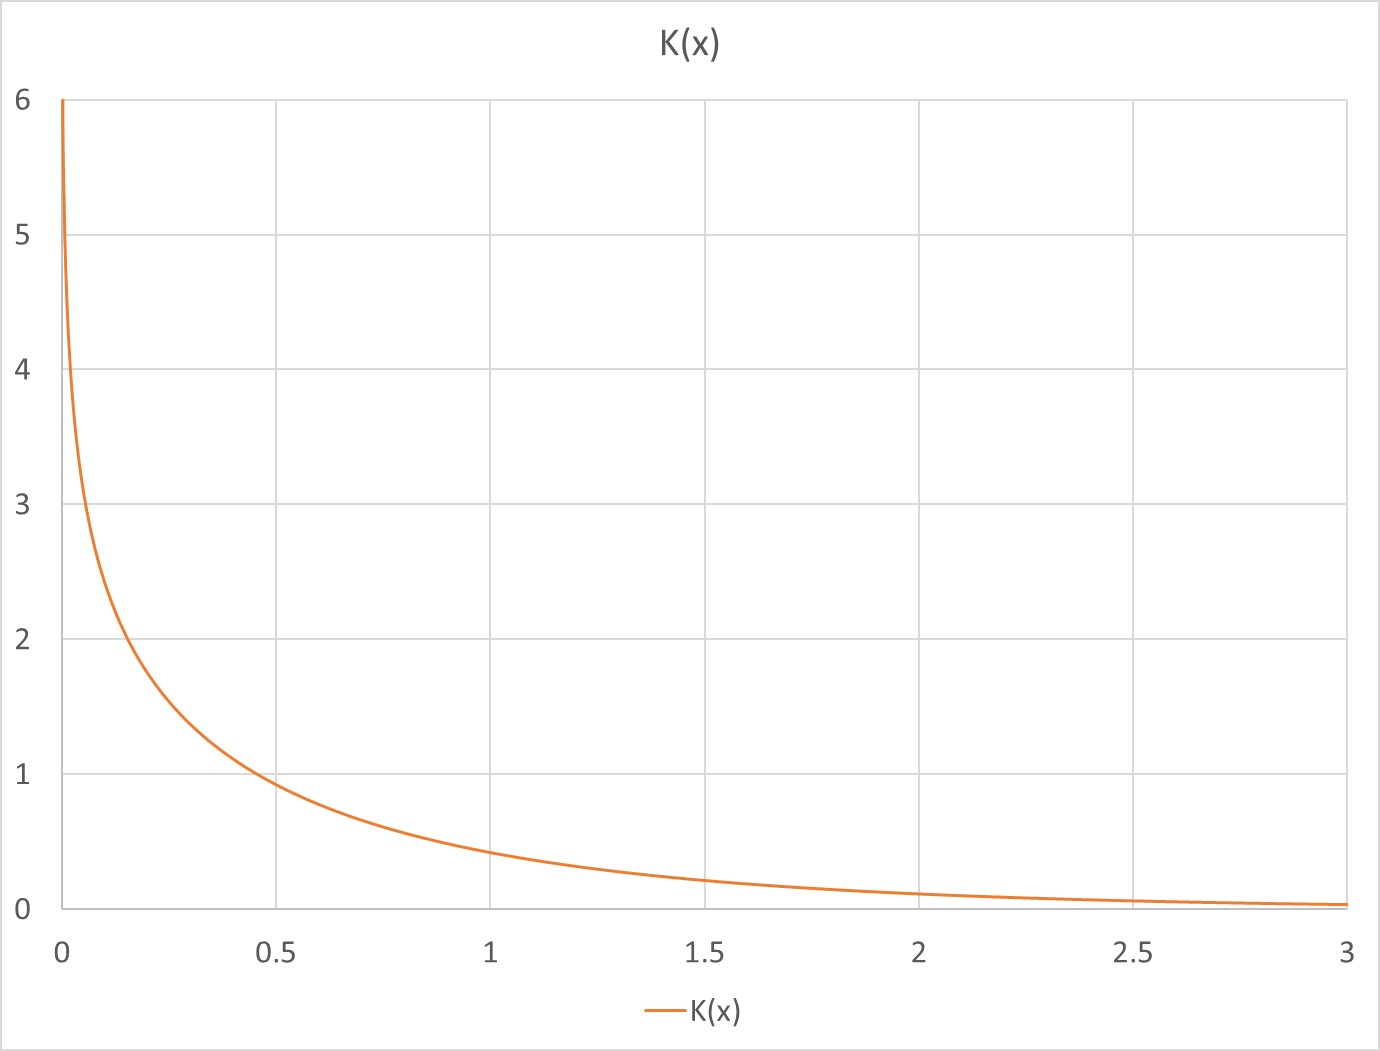
\includegraphics[width=.8\linewidth]{K_bessel}
\end{figure}


Based on the figure, it shows that $x\rightarrow 0$, then $K_0 = \infty$, hence, $C$ must be zero.
\bigbreak
Apply BC2:
\begin{align*}
    0 &= J^-\bigg(\frac{T}{2}\bigg) = \frac{\phi\bigg(\frac{T}{2}\bigg)}{4}+\frac{D}{2}\phi'\bigg(\frac{T}{2}\bigg) \\
    0 &= 0.25\bigg[AI_0\bigg(B\frac{T}{2}\bigg)+\frac{S_0}{\Sigma_a}\bigg]+\frac{D}{2}B\bigg[AI_1\bigg(B\frac{T}{2}\bigg)\bigg] \\
    0 &= A\bigg[I_0\bigg(B\frac{T}{2}\bigg)+2DBI_1\bigg(B\frac{T}{2}\bigg)\bigg]+\frac{S_0}{\Sigma_a} \\
    A &= -\frac{\frac{S_0}{\Sigma_a}}{I_0(B\frac{T}{2})+2DBI_1(B\frac{T}{2})}
\end{align*}


The flux in the cylinder is:
\boxed{
\begin{equation*}
    \phi(r) = \frac{S_0}{\Sigma_a}\bigg[1-\frac{I_0(Br)}{I_0(B\frac{T}{2})+2DBI_1(B\frac{T}{2})}\bigg]
\end{equation*}
}

%###############################################################################
% part (c)
%###############################################################################

(c) The approximate form of the diffusion equation for a spherical reactor is given below:
\bigbreak
\begin{equation*}
    \frac{1}{r^2}\frac{d}{dr}\bigg(r^2 \frac{d\phi(r)}{dr}\bigg) +B^2\phi(r) + \frac{S(r)}{D} = 0
\end{equation*}

\begin{figure}[h!]
    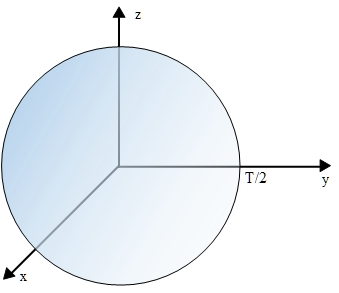
\includegraphics[width=.45\linewidth]{P1c}
\end{figure}
\bigbreak


The general form of the solution:
\bigbreak
\[   \phi(r) = \left\{
\begin{array}{ll}
      A\frac{e^{Br}}{r} + C\frac{e^{-Br}}{r}, &  B^2 < 0\\
      A\frac{\sin(Br)}{r} + C\frac{\cos(Br)}{r}, &  B^2 > 0\\
\end{array}
\right. \]
\bigbreak


The boundary conditions for this geometry are given below:
\begin{itemize}
    \item $\lim_{r \rightarrow 0}Jr4\pi r^2$ = 0
    \item $J^-$(T/2) = $J^+$(-T/2) = 0
    \item $\phi(0) \neq \infty$
    \item $\lim_{x\to\infty} \phi(x)$ = 0
\end{itemize}


Instead of using the above general solution for $B^2 < 0$, a general solution using $\sinh$ and $\cosh$ can be developed:
\begin{equation*}
    \phi(r) = \frac{A\sinh(Br)}{r}+\frac{C\cosh(Br)}{r}+\frac{S_0}{\Sigma_a}
\end{equation*}


Apply BC1, and the equation $Jr = -D\phi'$:
\begin{align*}
    0 &= -4D\pi[A(B(0)\cosh(B(0))-\sinh(B(0)))+C(B(0)\sinh(B(0))-\cosh(B(0)))] \\
    0 &= -4D\pi C \\
    C &= 0
\end{align*}


Apply BC2:
\begin{align*}
    0 &= J^-\bigg(\frac{T}{2}\bigg) = \frac{\phi\bigg(\frac{T}{2}\bigg)}{4} +\frac{D}{2}\phi'\bigg(\frac{T}{2}\bigg) \\
    0 &= 0.25\Bigg[\frac{A\sinh\bigg(B\frac{T}{2}\bigg)}{\frac{T}{2}}+\frac{S_0}{\Sigma_a}\Bigg] +\frac{D}{2}\Bigg[\frac{A\bigg[B\bigg(\frac{T}{2}\bigg)\cosh\bigg(B\bigg(\frac{T}{2}\bigg)\bigg)-\sinh\bigg(B\bigg(\frac{T}{2}\bigg)\bigg)\bigg]}{\bigg(\frac{T}{2}\bigg)^2}\Bigg] \\
    0 &= A\Bigg[\frac{\sinh\bigg(B\frac{T}{2}\bigg)}{\frac{T}{2}}+\frac{2D\bigg[B\bigg(\frac{T}{2}\bigg)\cosh\bigg(B\bigg(\frac{T}{2}\bigg)\bigg)-\sinh\bigg(B\bigg(\frac{T}{2}\bigg)\bigg)\bigg]}{\bigg(\frac{T}{2}\bigg)^2}\Bigg]+\frac{S_0}{\Sigma_a} \\
    A &= -\frac{\frac{S_0}{\Sigma_a}}{\frac{\sinh\bigg(B\frac{T}{2}\bigg)}{\frac{T}{2}}+\frac{2D\bigg[B\bigg(\frac{T}{2}\bigg)\cosh\bigg(B\bigg(\frac{T}{2}\bigg)\bigg)-\sinh\bigg(B\bigg(\frac{T}{2}\bigg)\bigg)\bigg]}{\bigg(\frac{T}{2}\bigg)^2}}
\end{align*}


Solution for the flux in the sphere:
\bigbreak
\boxed{
\begin{equation*}
    \phi(r) = \frac{S_0}{\Sigma_a}\Bigg[1-\frac{\sinh(Br)}{r}\frac{1}{\bigg(\frac{\sinh(B\frac{T}{2})}{\frac{T}{2}}+\frac{2D[B(\frac{T}{2})\cosh(B(\frac{T}{2}))-\sinh(B(\frac{T}{2}))]}{(\frac{T}{2})^2}\bigg)}\Bigg]
\end{equation*}
}


%###############################################################################
%  part (d)
%###############################################################################
(d) The approximate form of the diffusion equation for this system:
\bigbreak

\begin{equation*}
    \frac{d^2}{dx^2}\phi(x) + B^2\phi(x) = S(x)
\end{equation*}
 
\begin{figure}[h!]
    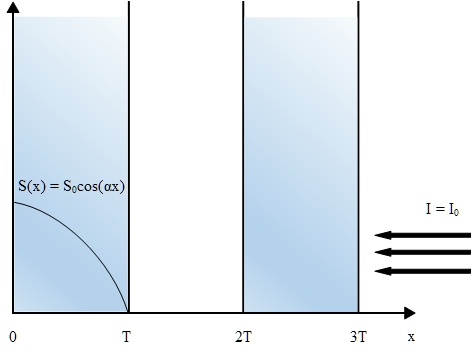
\includegraphics[width=.45\linewidth]{P1d}
\end{figure}
\bigbreak


The solution general form:
\bigbreak
\[   \phi(x) = \left\{
\begin{array}{ll}
      Ae^{-Bx} + Ce^{Bx} &  \\
      A'\sinh(Bx) + C'\cosh(Bx) &  \\
\end{array}
\right. , \quad B^2 < 0\]
\bigbreak
\[   \phi(x) = \left\{
\begin{array}{ll}
      Ae^{-iBx} + Ce^{iBx} &  \\
      A'\sin(Bx) + C'\cos(Bx) &  \\
\end{array}
\right. , \quad B^2 > 0\]
\bigbreak


The boundary conditions:
\begin{itemize}
    \item $J^+$(T) = $J^+$(2T)
    \item $J^-$(T) = $J^-$(2T)
    \item $\lim_{x \to \infty} \phi(x)$ = 0
\end{itemize}
\bigbreak




%%%%%%%%%%%%%%%%%%%%%%%%%%%%%%%%%%%%%%%%%%%%%%%%%%%%%%%%%%%%%%%%%%%%%%%%%%%%%%%%%%%%%%%%%%%%%%%%%%%%%%%%%%%%%%%%%%%%%%%%%%%
%                                                         PROBLEM 2
%%%%%%%%%%%%%%%%%%%%%%%%%%%%%%%%%%%%%%%%%%%%%%%%%%%%%%%%%%%%%%%%%%%%%%%%%%%%%%%%%%%%%%%%%%%%%%%%%%%%%%%%%%%%%%%%%%%%%%%%%%%

\newpage

\textbf{Problem 2:} Write a computer program to calculate the steady-state flux density distribution in a homogeneous infinite slab, sphere, and infinite cylinder each of which may contain an arbitrarily distributed volumetric source of neutrons.
Assume vacuum boundary conditions.
\bigbreak

(a) Derive the first-order finite-difference form of the appropriate one-speed diffusion equation.
Assume equal mesh spacing.\newline
\bigbreak

(b) Write the resulting equations in matrix form \textbf{$A\phi$} = \textbf{$s$}.\newline
\bigbreak

(c) Derive the TDMA algorithm to solve this set of equations and write a subroutine to implement this algorithm.\newline
\bigbreak

(d) Write a program to solve the 1-D finitie-difference diffusion equations developed in part (a).
Input should include: geometry type, system size, number of mesh points desired, parameters $\Sigma_a$ and $D$, and the source distribution $S(r_i)$.\newline
\bigbreak

%%%%%%%%%%%%%%%%%%%%%%%%%%%%%%%%%%%%%%%%%%%%%%%%%%%%%%%%%%%%%%%%%%%%%%%%%%%%%%%%%%%%%%%%%%%%%%%%%%%%%%%%%%%%%%%%%%%%%%%%%%%

\textbf{Solution}
\bigbreak
(a) The following image shows how meshing works for the finite difference method.
\bigbreak


% finite difference image
\begin{figure}[h!]
    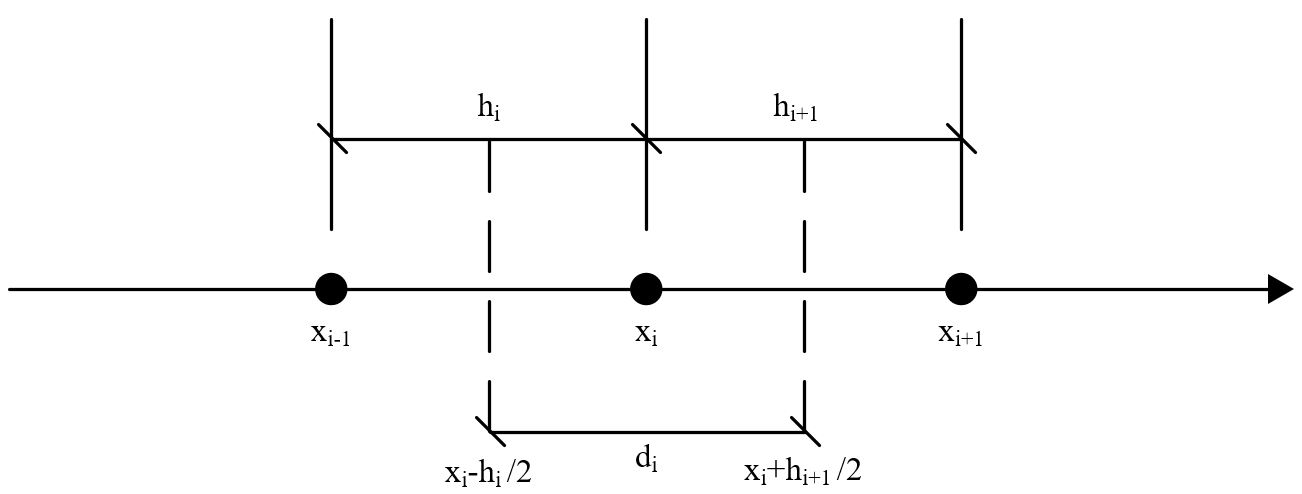
\includegraphics[width=.7\linewidth]{FD2}
\end{figure}


In our analysis, we will assume that each node is equally spaced.
We begin with the 1-D diffusion equation for each of the geometries.


\begin{align*}
    S(x) &= -D\frac{d^2}{dx^2}\phi(x) + \Sigma_a\phi(x), \quad &(slab)  \\
    S(x) &= -D\frac{d^2}{dx^2}\phi(x) + \frac{1}{x}\frac{d}{dx}\phi(x) +\Sigma_a\phi(x), \quad &(cylinder) \\
    S(x) &= -D\frac{1}{x^2}\frac{d}{dx}\bigg(x^2 \frac{d\phi(x)}{dx}\bigg) +\Sigma_a\phi(x), \quad &(sphere)
\end{align*}


This can be written in the following way by collapsing terms under a single constant $c$ determined by the particular geometry:

\begin{equation*}
    x^c S(x) = -D\frac{d}{dx}\bigg(x^c\frac{d\phi(x)}{dx}\bigg)+x^c\Sigma_a\phi(x)
\end{equation*}



In this form, the geometry determines the constant, $c$, where $c=0$ (slab), $c=1$ (cylinder), $c=2$ (sphere).

\begin{align*}
    \int_{x_i-d/2}^{x_i+d/2}dxS(x)x^c  &= -D\int_{x_i-d/2}^{x_i+d/2}dx\bigg[\frac{d}{dx}\bigg(x^c\frac{d\phi(x)}{dx}\bigg)\bigg]+\int_{x_i-d/2}^{x_i+d/2}dx \Sigma_a\phi(x)x^c \\
    S(x)x^cd &= -Dx^c\frac{d\phi(x)}{dx}\Biggr|_{x_i-d/2}^{x_i+d/2}+\Sigma_a\phi(x)x^cd \\
    S(x)x^cd &= -D(x_i+d/2)^c\bigg[\frac{\phi_{i+1}-\phi_i}{d}\bigg]+D(x_i-d/2)^c\bigg[\frac{\phi_i-\phi_{i-1}}{d}\bigg]+\Sigma_a\phi(x)x^cd
\end{align*}
\bigbreak



This yields the solution:
\boxed{S(x)x^cd =-D(x_i+d/2)^c\bigg[\frac{\phi_{i+1}-\phi_i}{d}\bigg]+D(x_i-d/2)^c\bigg[\frac{\phi_i-\phi_{i-1}}{d}\bigg]+\Sigma_a\phi(x)x^cd}


% begin part (b)
(b) The equation, $A\phi = s$, allows us to find the coefficients.
Dividing each term, from the previous part, by $x^cd$ gives the matrix form:
\bigbreak

% matrix form
\boxed{a_{i,i-1}\phi_{i-1}+a_{i,i}\phi_{i}+a_{i,i+1}\phi_{i+1}=S_i}
\bigbreak

where $a_{i,i-1}$, $a_{i,i}$, and $a_{i,i+1}$ are defined as:
\begin{align*}
    a_{i,i-1} &= -\frac{D}{d^2}\bigg(1-\frac{1}{2i}\bigg)^c \\
    a_{i,i} &= \Sigma_a+\frac{D}{d^2}\bigg[\bigg(1-\frac{1}{2i}\bigg)^c+ \bigg(1+\frac{1}{2i}\bigg)^c\bigg] \\
    a_{i,i+1} &= -\frac{D}{d^2}\bigg(1+\frac{1}{2i}\bigg)^c
\end{align*}
\bigbreak



(c) The matrix form below shows the TMDA algorithm:
\begin{figure}[h!]
    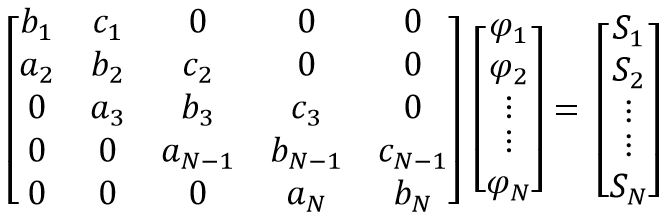
\includegraphics[width=.5\linewidth]{TDMA}
\end{figure}
\bigbreak


We begin with forward elimination, going from row 2 to N:
\begin{align*}
    m &= \frac{a_i}{b_{i-1}} \\
    b_i &= b_i - mc_{i-1} \\
    d_i &= d_i - md_{i-1}
\end{align*}

The following product series is found:
\begin{align*}
    b_i &= b_i - \prod_{i = 2}^{N} (a_i)^{-i^{(i-1)}} (b_{i-1})^{-i^{(i)}} (c_{i-1})^{-i^{(i-1)}}, \quad i>2 \\
    S_i &= S_i - \prod_{i = 2}^{N} (a_i)^{-i^{(i-1)}} (b_{i-1})^{-i^{(i)}} (S_{i-1})^{-i^{(i-1)}}, \quad i>2
\end{align*}

Then we apply backward substitution for rows n-1 to 1:
\begin{align*}
    \phi_i &= \frac{S_i}{b_i} \\
    \phi_i &= \frac{S_i-c_i\phi_{i+1}}{b_i}
\end{align*}

The following product series are found:
\begin{align*}
    b_i &= b_i - \prod_{i = 2}^{N} (a_i)^{-i^{(i-1)}} (b_{i-1})^{-i^{(i)}} (c_{i-1})^{-i^{(i-1)}}, \quad i>2 \\
    S_i &= S_i - \prod_{i = 2}^{N} (a_i)^{-i^{(i-1)}} (b_{i-1})^{-i^{(i)}} (S_{i-1})^{-i^{(i-1)}}, \quad i>2
\end{align*}
 

%%%%%%%%%%%%%%%%%%%%%%%%%%%%%%%%%%%%%%%%%%%%%%%%%%%%%%%%%%%%%%%%%%%%%%%%%%%%%%%%%%%%%%%%%%%%%%%%%%%%%%%%%%%%%%%%%%%%%%%%%%%
%                                                         PROBLEM 3
%%%%%%%%%%%%%%%%%%%%%%%%%%%%%%%%%%%%%%%%%%%%%%%%%%%%%%%%%%%%%%%%%%%%%%%%%%%%%%%%%%%%%%%%%%%%%%%%%%%%%%%%%%%%%%%%%%%%%%%%%%%

\newpage
\textbf{Problem 3:} Use your program to solve the first three problems of question 1.
Data to be used are: $D$ = 0.600 cm, $\Sigma_a$ = 0.005 $cm^{-1}$, $T$ = 45 cm, and $S_0$ = $10^8$ neutrons cm${}^{-2}$ s${}^{-1}$.
Plot both the numerical solution and the analytical flux profile for each problem.
Also investigate the effect of mesh size on the accuracy of the solutions.

\bigbreak
%%%%%%%%%%%%%%%%%%%%%%%%%%%%%%%%%%%%%%%%%%%%%%%%%%%%%%%%%%%%%%%%%%%%%%%%%%%%%%%%%%%%%%%%%%%%%%%%%%%%%%%%%%%%%%%%%%%%%%%%%%%
\textbf{Solution}

Using the parameters described in the problem statement, the code created in problem 2 was used to approximate a solution to (a) - (b) in problem 1.
The following plots show these solutions, for $n=10$, $n=100$, and $n=1000$.
It can be seen that as $n$ is increased, the approximation is much more accurate.
In the slab problem, the solution seems to be a decent approximation for the $n=10$ case; however, for the other two cases, a large $n$ is necessary for convergence on a good solution.


% slab finite diff image
\begin{figure}[h!]
    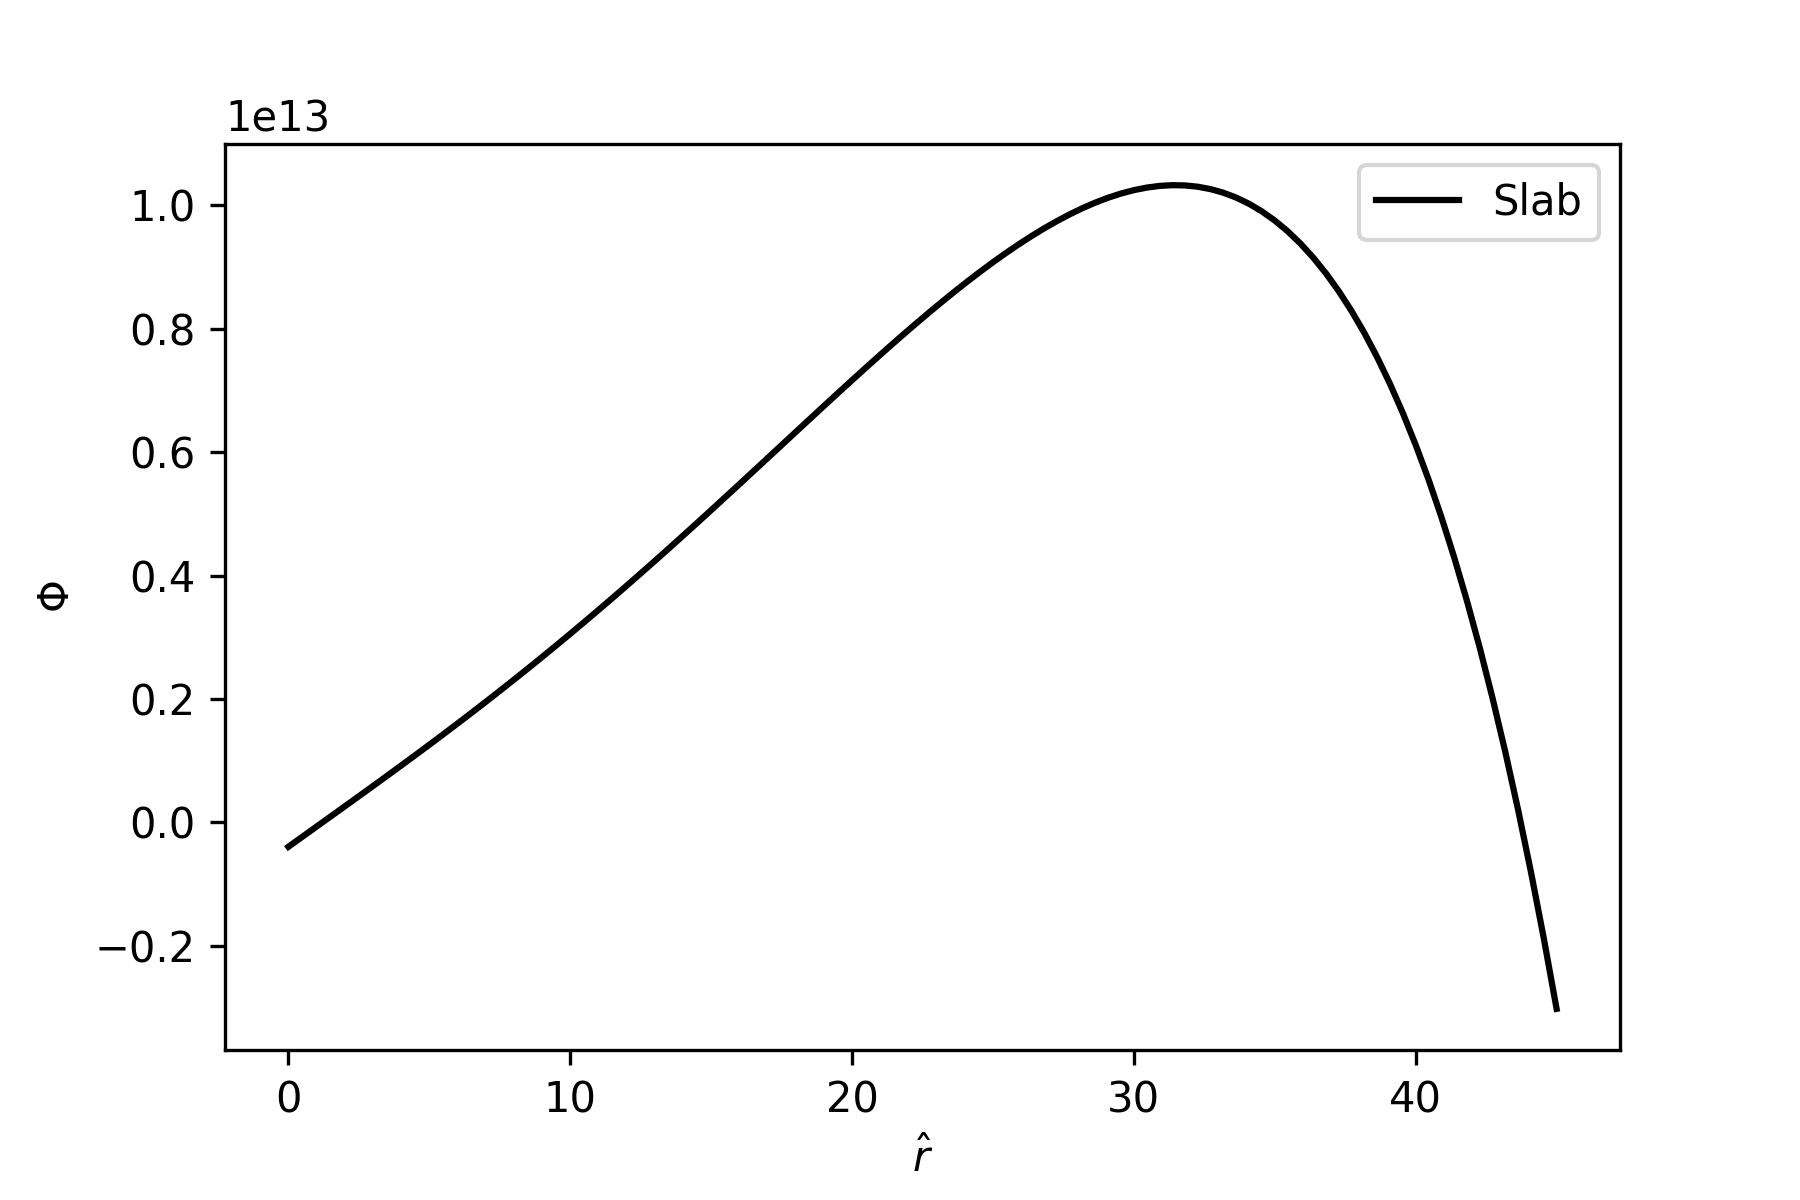
\includegraphics[width=.7\linewidth]{slab}
\end{figure}

% cylinder finite diff image
\begin{figure}[h!]
    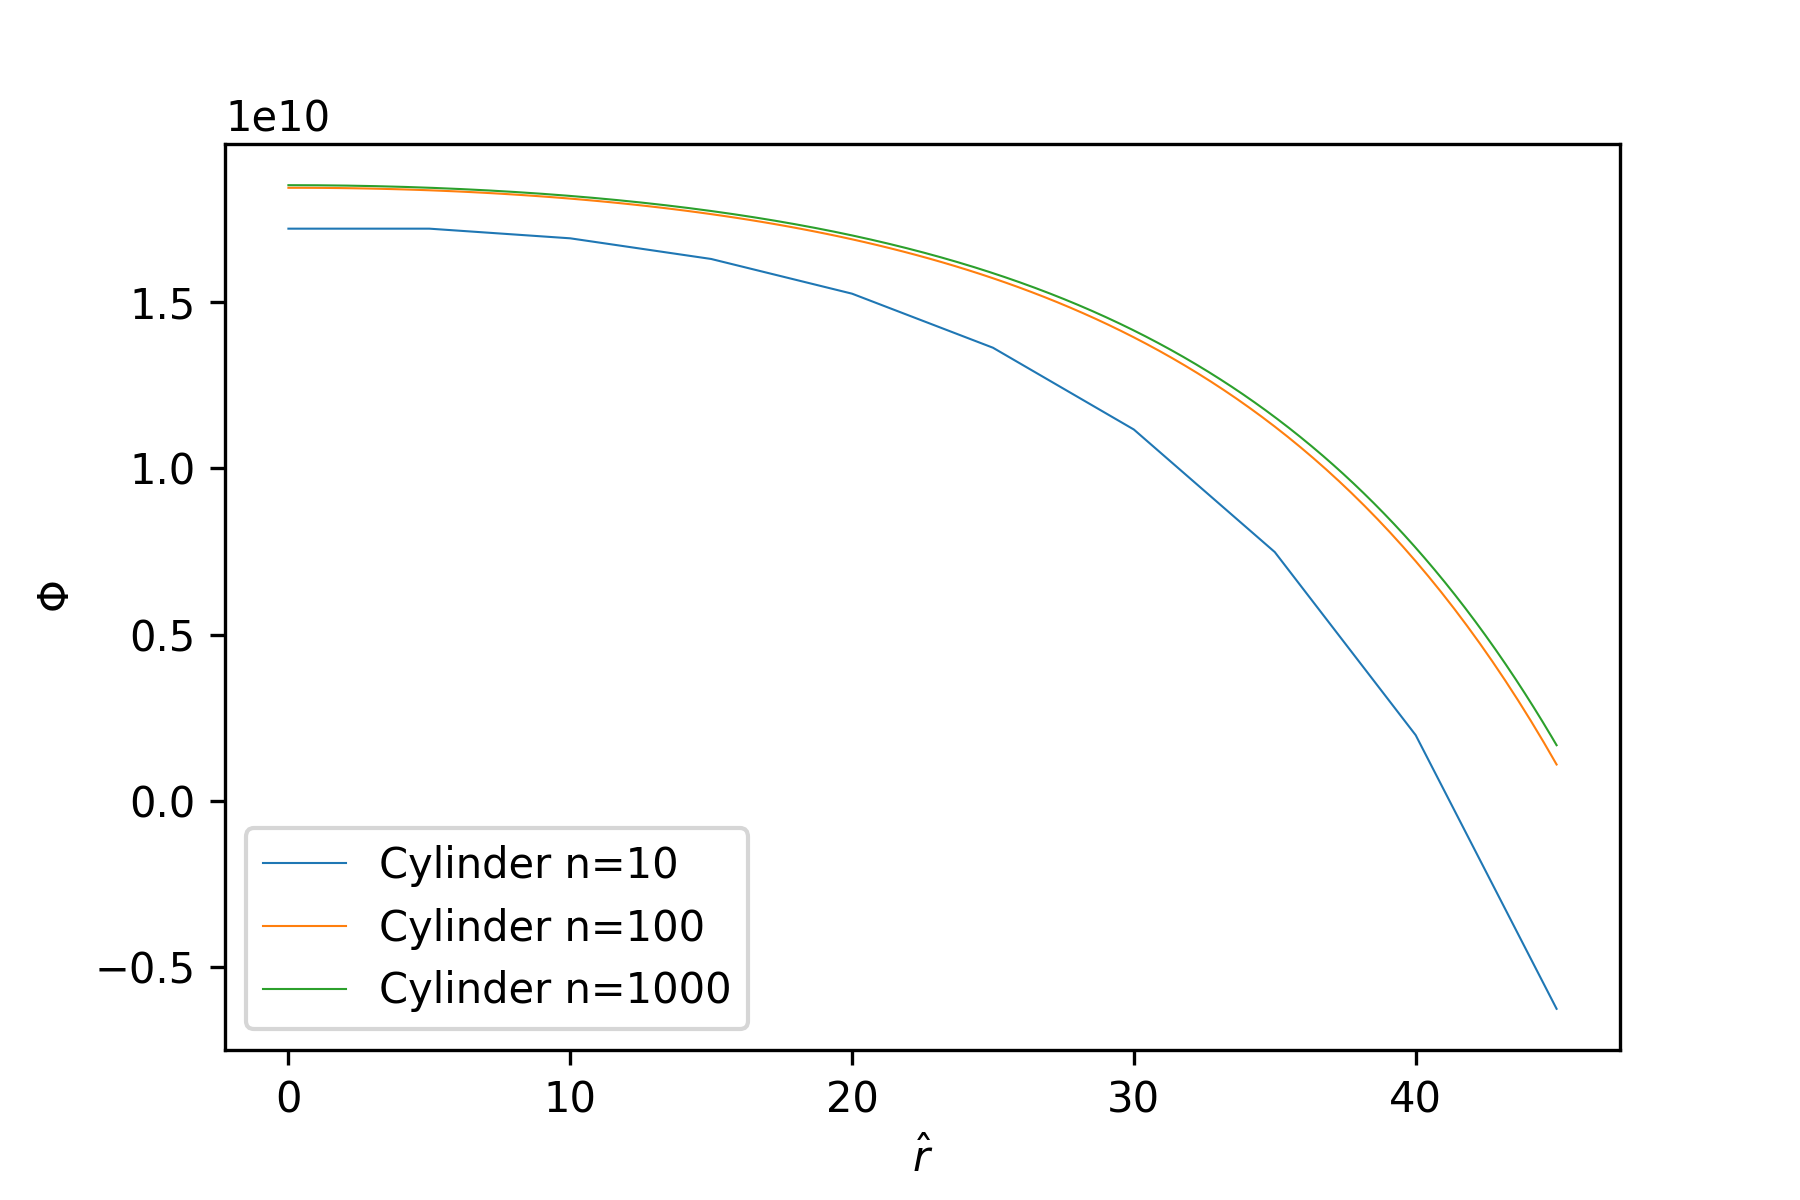
\includegraphics[width=.7\linewidth]{cyl}
\end{figure}

% spherical finite diff image
\begin{figure}[h!]
    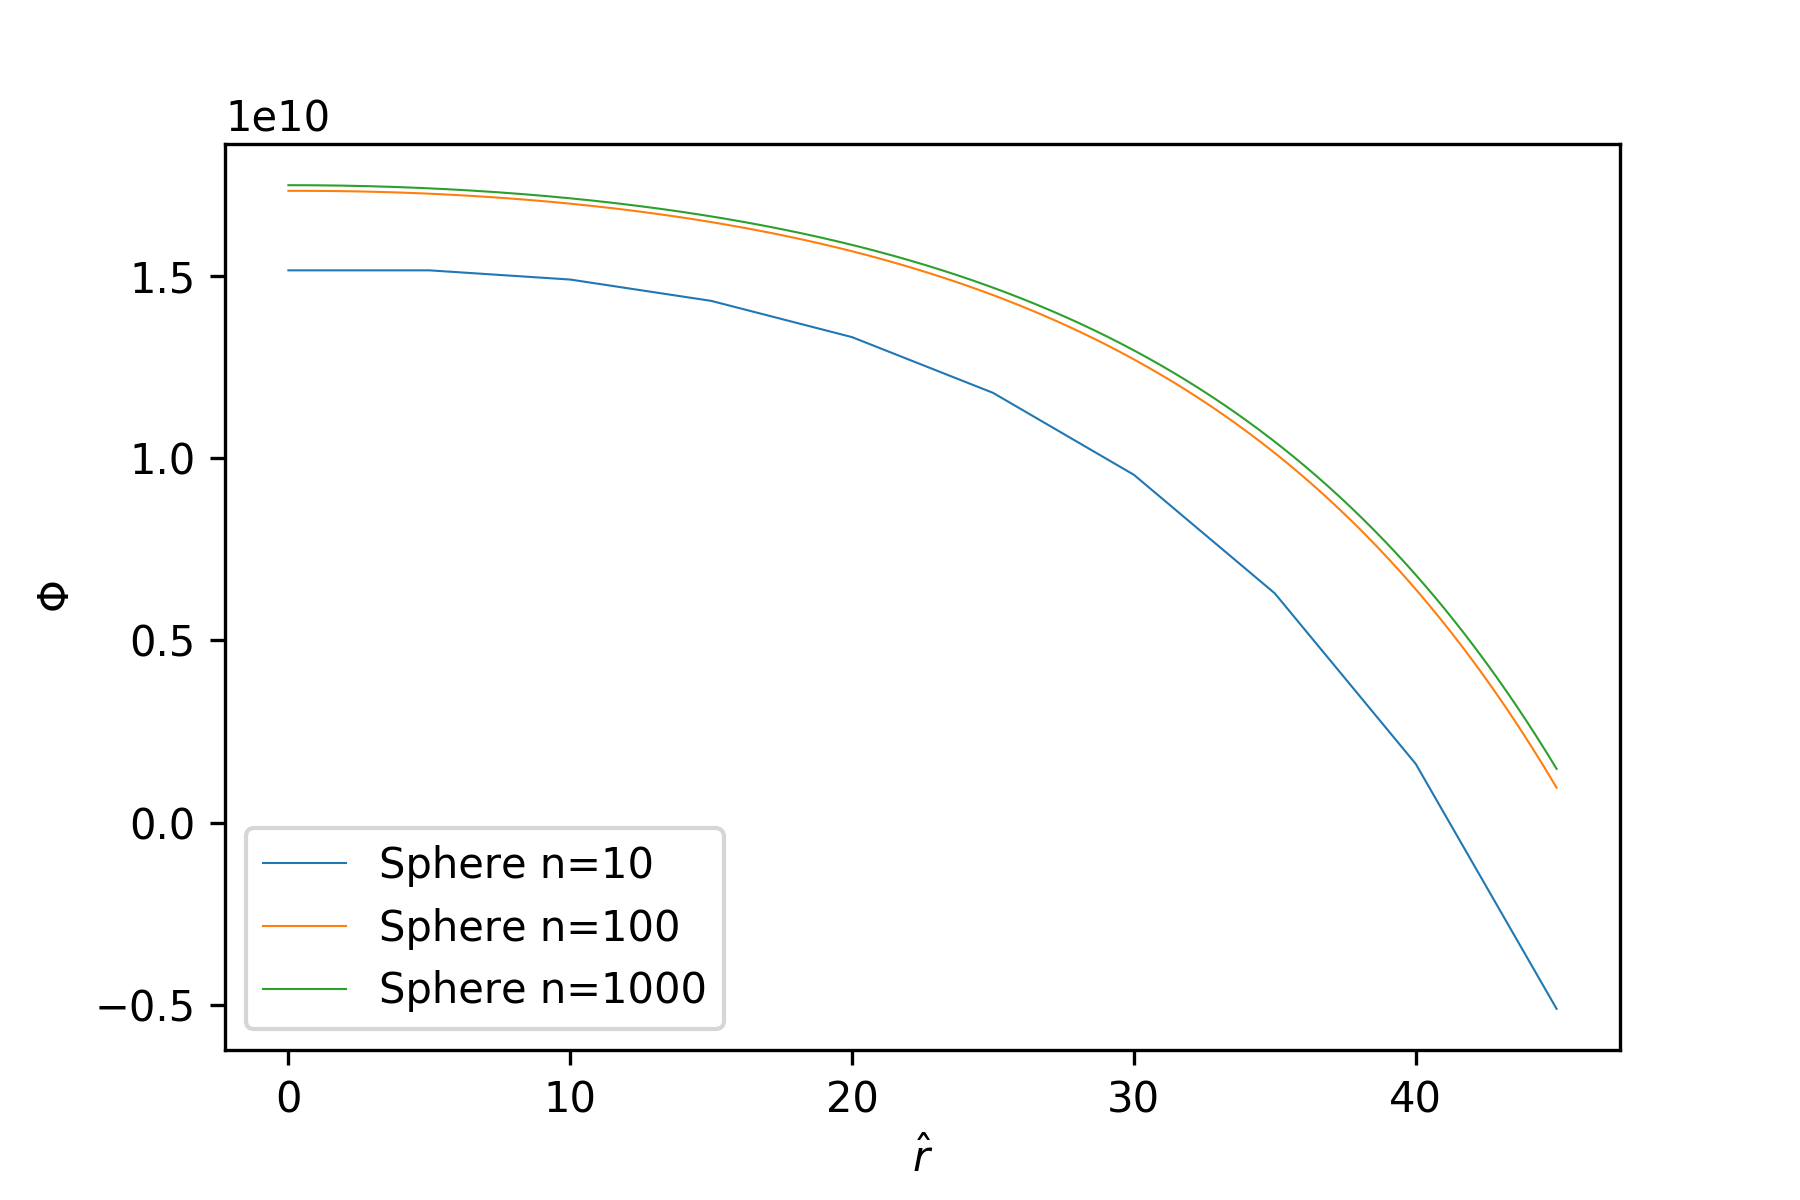
\includegraphics[width=.7\linewidth]{sph}
\end{figure}

 
\bigbreak
%%%%%%%%%%%%%%%%%%%%%%%%%%%%%%%%%%%%%%%%%%%%%%%%%%%%%%%%%%%%%%%%%%%%%%%%%%%%%%%%%%%%%%%%%%%%%%%%%%%%%%%%%%%%%%%%%%%%%%%%%%%
\end{document}
